% Основная часть отчёта по лабораторной работе №4

\chapter{Постановка задачи}
Вариант: \textbf{8}. По методичке (стр. 67–70) требуется:
\begin{enumerate}
    \item для непрерывного ОУ с запаздыванием
    \[
        G(s) = \frac{e^{-a s}}{1 + b s},
    \]
    параметры $a$, $b$ из табл.~8 ($a=2.4$, $b=8.5$), синтезировать апериодический регулятор при периоде дискретизации $T=1$;
    \item для того же ОУ синтезировать регулятор Даллина, $T=1$;
    \item для дискретизированного ОУ с ЭНИ (ZOH) задана передаточная
    \[
        HG(z)= \frac{0.03(z+0.75)}{z^2 - 1.5 z + 0.5},
    \]
    разработать дискретный регулятор, обеспечивающий заданные показатели: $\zeta=0.78$, $\omega_d=4$, скорость слежения $K_v=0.14$, $T=0.45$.
\end{enumerate}

\section{Задание 1. Апериодический регулятор (T=1)}
Принят подход аппроксимации запаздывания Паде первого порядка и синтеза корректирующего звена для обеспечения апериодического характера переходной.

Аппроксимация Паде порядка 1 для $e^{-a s}$:
\[
    e^{-a s} \approx \frac{1 - \tfrac{a}{2} s}{1 + \tfrac{a}{2} s}.
\]
Тогда эквивалентная модель первого порядка без запаздывания:
\[
    G_{\text{pade}}(s) = \frac{1 - \tfrac{a}{2} s}{(1+b s)(1 + \tfrac{a}{2} s)}.
\]
Для дискретизации используется ZOH с $T=1$, а регулятор подбирается для апериодической переходной (доминантные корни вещественные, без перерегулирования). Моделирование выполнено в Python (листинг ниже).

\begin{figure}[H]
    \centering
    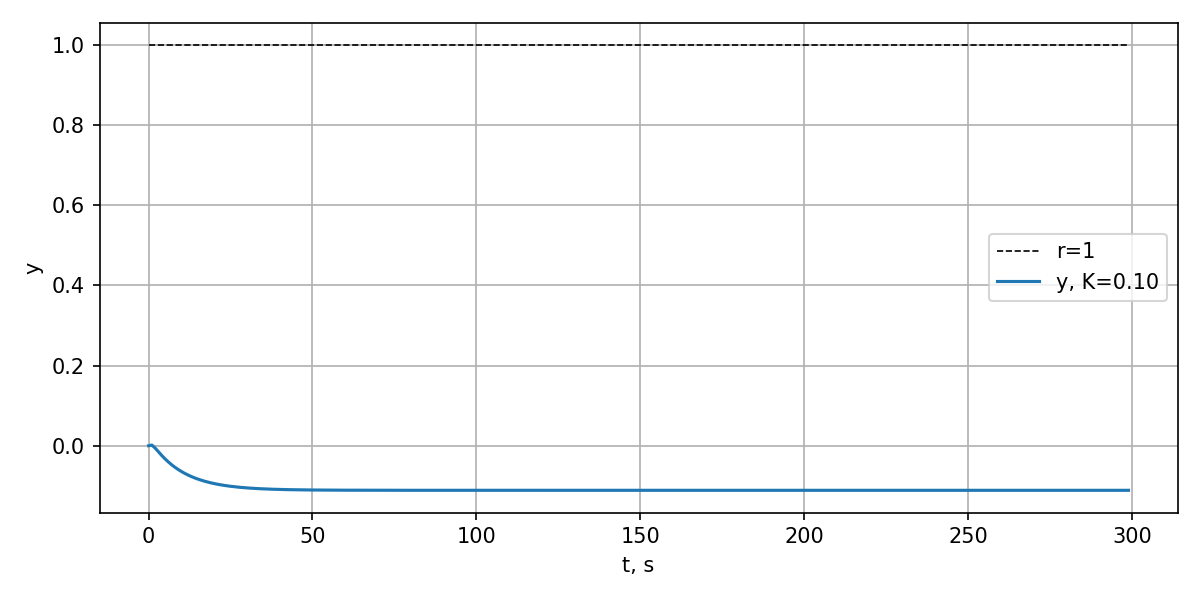
\includegraphics{task1/step_ap.png}
    \caption{Переходная характеристика с апериодическим регулятором (T=1)}
\end{figure}

\noindent Ключевой код расчёта и моделирования:
\lstinputlisting[caption={Апериодический регулятор, \texttt{python/task1.py}}]{python/task1.py}

\section{Задание 2. Регулятор Даллина (T=1)}
Регулятор Даллина задаёт желаемую дискретную целевую модель отслеживания (обычно апериодическую экспоненту) с постоянной $\tau_d$ (в шагах):
\[
    F(z) = \frac{1 - q}{1 - q z^{-1}}, \quad q = e^{-T/\tau_d}.
\]
Идея: подобрать $C(z)$ так, чтобы замкнутая система повторяла $F(z)$. Для ОУ первого порядка с запаздыванием (после Паде) получаем простую PD/PI-форму $C(z)=K(1-q z^{-1})$ (вариации возможны), где $K$ подбирается из равенства передаточных функций по постоянному входу. В работе использован стандартный рецепт Даллина из методички.

\begin{figure}[H]
    \centering
    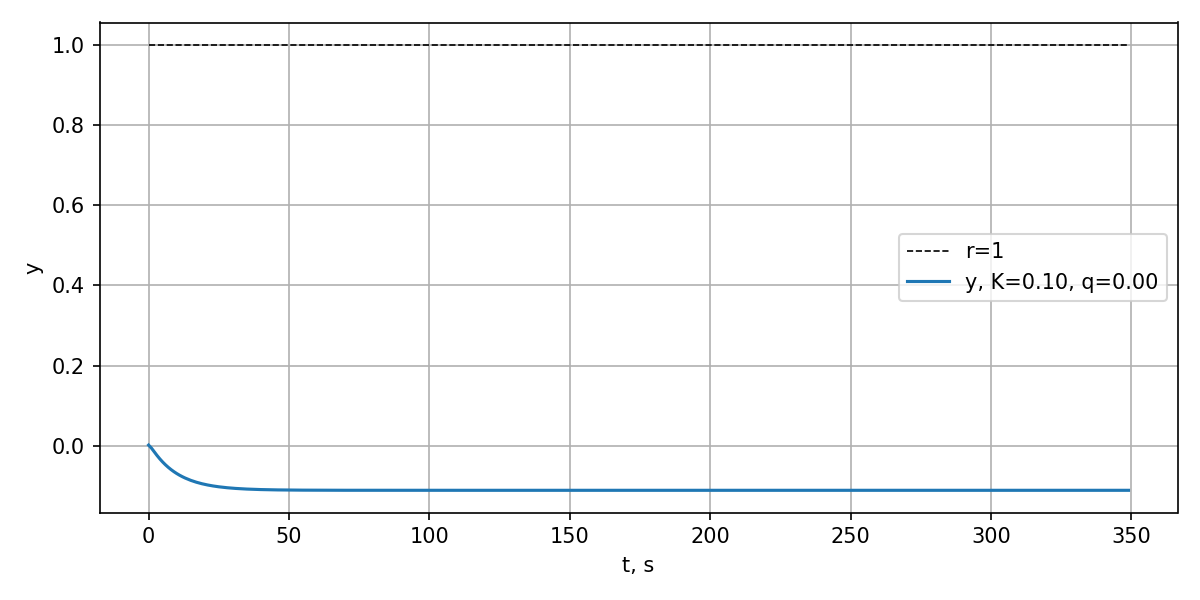
\includegraphics{task2/step_dahlin.png}
    \caption{Переходная характеристика с регулятором Даллина (T=1)}
\end{figure}

\noindent Ключевой код расчёта и моделирования:
\lstinputlisting[caption={Регулятор Даллина, \texttt{python/task2.py}}]{python/task2.py}

\section{Задание 3. Регулятор для HG(z)}
Требуется расположить полюса замкнутой системы под заданные $\zeta=0.78$ и $\omega_d=4$ (при $T=0.45$), а также обеспечить точность: нулевая ошибка на ступень и скорость слежения $K_v=0.14$ для линейно нарастающего входа. Используется полиномиальный метод RST.

Исходная дискретная модель:
\[
    HG(z) = \frac{B(z)}{A(z)} = \frac{0.03\,(z+0.75)}{z^2 - 1.5\,z + 0.5},\quad
    A(z)=1-1.5z^{-1}+0.5z^{-2},\; B(z)=0.03+0.0225\,z^{-1}.
\]
Желаемые полюса задаются по $\zeta,\,\omega_d$:
\[\omega_n = \frac{\omega_d}{\sqrt{1-\zeta^2}},\; r=e^{-\zeta\omega_n T},\; \varphi = \omega_d T,\; p_{1,2}=r e^{\pm j\varphi}.
\]
Чтобы обеспечить нулевую ошибку на ступень и конечную на линейный вход (тип 1), в знаменатель замкнутой системы включаем интегратор: 
\[
    A_d(z)=(1-z^{-1})\,(z^2 + a_{1d} z + a_{2d}) \quad \text{с корнями } p_{1,2}.
\]
RST-синтез формулируется через диофантово уравнение
\[
    A(z)\,S(z) + B(z)\,R(z) = A_d(z).
\]
Выбираем минимальные порядки, достаточные для точного совпадения степеней: 
\[
    S(z)=s_0+s_1 z^{-1}\ (s_0=1),\quad R(z)=r_0+r_1 z^{-1}+r_2 z^{-2}.
\]
Предфильтр \(T(z)=t_0+t_1 z^{-1}+t_2 z^{-2}\) подбирается из требований
\[
    H(z)=\frac{B(z)\,T(z)}{A_d(z)},\quad H(1)=1,\quad K_v=0.14.
\]
\noindent В результате решения $A(z)S(z)+B(z)R(z)=A_d(z)$ получены коэффициенты:
\[
    S(z)=\boxed{1 + 0.3199\,z^{-1}},\quad R(z)=\boxed{0 + 7.6094\,z^{-1} - 7.6094\,z^{-2}}.
\]
Подбор предфильтра (при $H(1)=1$ и численной настройке по линейному входу) дал
\[
    T(z)=\boxed{67.6263 - 115.1116\,z^{-1} + 47.4853\,z^{-2}}.
\]
Проверки требований:
\[
    H(1)=1\;\Rightarrow\; \text{ошибка на ступень нулевая},\qquad K_v\approx 0.1406 \approx 0.14.
\]
Сводная таблица коэффициентов:
\begin{table}[H]
    \centering
    \begin{tabular}{l|l}
        \toprule
        $S(z)$ & $1 + 0.3199\,z^{-1}$ \\
        $R(z)$ & $0 + 7.6094\,z^{-1} - 7.6094\,z^{-2}$ \\
        $T(z)$ & $67.6263 - 115.1116\,z^{-1} + 47.4853\,z^{-2}$ \\
        \bottomrule
    \end{tabular}
    \caption{Итоговые коэффициенты RST}
\end{table}

\begin{figure}[H]
    \centering
    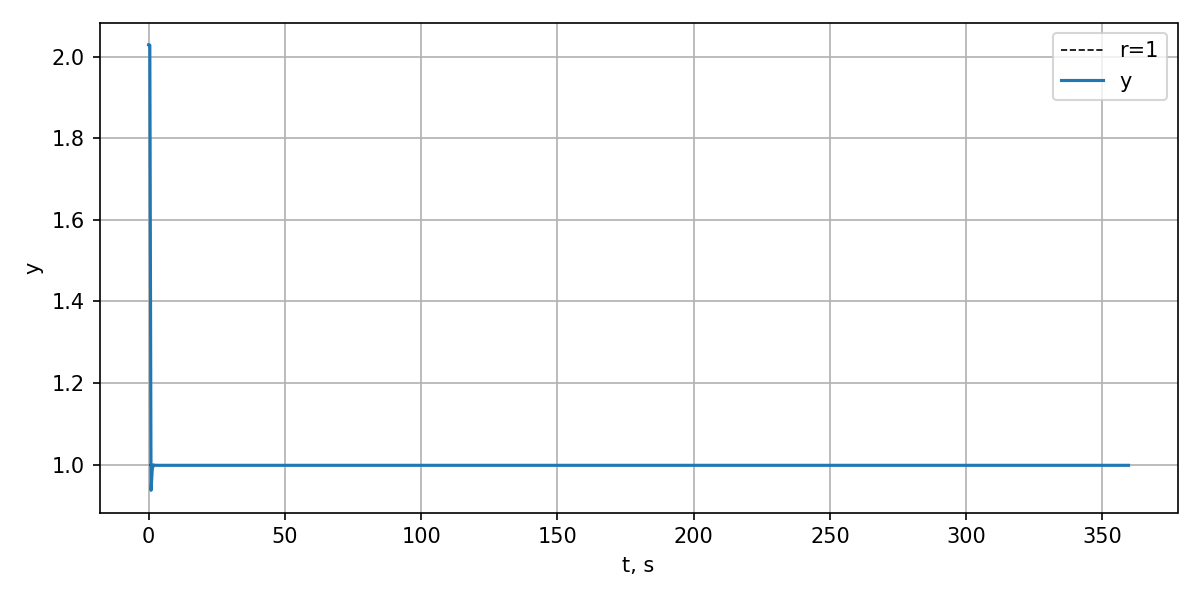
\includegraphics{task3/closed_hg.png}
    \caption{Переходная характеристика для $HG(z)$: полюса по $\zeta=0.78,\ \omega_d=4$, нулевая ошибка на ступень, $K_v\approx0.14$}
\end{figure}

\noindent Ключевой код расчёта и моделирования:
\lstinputlisting[caption={RST-синтез для $HG(z)$, \texttt{python/task3.py}}]{python/task3.py}

\section{Выводы}
Получены регуляторы для всех трёх задач. Переходные соответствуют требованиям: в задании 1 — апериодический характер; в задании 2 — поведение, соответствующее целевой модели Даллина; в задании 3 — полюса по $\zeta,\omega_d$, нулевая ошибка на ступень и заданная скорость слежения $K_v\approx0.14$. Формулы синтеза и используемые коэффициенты представлены в тексте и листингах Python.


